\chapter{Relation Extraction Engine}

This section focuses on the relation extraction engine, covering the journey to the current implementation, focusing on data preparation and the different approaches for extracting semantic triples.

\section{Data Pre-Processing}

Before the relations are extracted from the articles, the articles need to be processed. This involves the coreference resolution and data cleaning to remove stopwords, unnecessary punctuation etc. as discussed in previous sections \ref{coref} and \ref{data_cleaning} respectively. Pre-processing the articles with coreference resolution has the benefit that all the \hl{............}

\todonum[inline]{add stuff}

\section{Motivation}
The motivation behind this \hl{part of the project} was to find a way to extract meaningful information from the article, in particular, information centred around key entities in the article corpus for a certain topic. This subsection covers the two different ideas explored for extracting information from articles. 

\subsection{Cooccurence Graph}
One of the earlier approaches was to derive a co-occurrence graph from the article corpus (pre-processed with coreference resolution and data cleaning) for a selected topic. This was useful in showing what entities were present and how they connected to one another as shown in \hl{Figure} \ref{coocc}. In order to derive the cooccurence graph, Named Entity Recognition (NER) was used. For each article, the \hl{intro} sentences were extracted and on each sentence NER was performed to extract all relevant entities. The types of entities extracted included but were not limited to, 'GPE', 'PER', 'LOC', 'ORG' etc. and excluded 'DATE', 'MONEY', 'TIME', 'CARDINAL', 'PERCENT' and 'QUANTITY' \hl{(See Appendix for reference)}. As seen in Figure \ref{coocc} in Appendix, the the size of the nodes representing the entities were reflective of the number of co-occurrence links (edges) incident to and from other entities. This was done so that for any given topic the most relevant entities, i.e., mentioned the most in the group of articles representing a topic, was apparent. The \textbf{limitation} of this approach, was that while this was a good indicator of general entities talked about in a topic, the amount of information extracted from the topic article corpus was not sufficient and did not provide any explicit information about \textit{'how'} the entities were related to one another, but rather, just simply, that they were.

\subsection{Semantic Triples}
In an attempt to extract more 'relevant' information indicative to the content discussed in articles of a given topic, the decision was made to extract semantic triples from article corpus instead of building a cooccurrence graph. 
This involved finding subject-relation-object triples form the sentences in the article corpora. \hl{??????? better semantic information extraction}
\todonum[inline]{Talk about why the pure dependency parsing method did not go well}
The process of extracting these relations involved inferring both syntactic and semantic dependencies between tokens in a sentence, making use tokenisation, dependency parsing,  part-of-speech tagging and named entity recognition.

\section{Key decisions} \label{key_decisions_rel}
\hl{In order to capture better nodes and relations, phrases are used instead of words. Given an example of teh sentence in figure, are calling for gives better understanding than calling. Also talk about how the knowledge graph is the goal and in particular we want to see the subject as entities to find out all the information about them in articles in a topic.}

\subsection{Relation as verb phrases}

\subsection{Subject as entities} \label{subject_ents}
Given that the end goal is to build a knowledge graph, the nodes must have \hl{common entities so that the graph can display all the different triples about an entity and which entities exist in the article corpus of a given topic. Give an example. For example, having two triples one with subject British Airways and other will British Airways spokesperson is not ideal as both triples provide information about the entity British Airways, however, they will be displayed as discrete triples. Instead, splitting the subject phrase as } 
\subsection{Object as noun phrases}


\section{Implementation}

The semantic triples need to be of type subject-relation-object triples. The section highlights the how the subject, relation, object phrases were extracted from the articles in order to build a knowledge from these triples. 

\subsection{Extracting Verb Phrases}

As mentioned in Section \ref{key_decisions_rel}, the relation phrases would be extracted as verb phrases. First and foremost, the coreference resolved and cleaned articles are split into sentences and the verb phrases are extracted from each sentence. This is done by regex matching of part-of-speech tags as seen below. 
\begin{minted}{python}
verb_patterns = [[{'POS':'AUX', 'OP': '?'}, {"POS":"VERB"}, {"POS":"ADP"}], 
          [{'POS': 'VERB', 'OP': '?'}, {'POS': 'ADV', 'OP': '*'},
           {'POS': 'VERB', 'OP': '+'}],
           [{'POS': 'VERB', 'OP': '+'}] ,
           [{'POS': 'AUX', 'OP': '?'}, {'POS': 'PART', 'OP': '?'},
           {'POS': 'VERB', 'OP': '+'}]]
\end{minted}

\todonum[inline]{Talk about why these particular regex -how extracted pos- give examples}

Once the relevant verb phrases in a sentence are extracted, they are filtered to obtain the phrases where the root of the sentence is present. This is done by using dependency parsing through the SpaCy library. Generally, in dependency-based grammars, all words or tokens, in a sentence,  barring one,  are dependant on other words.  This is the root  of the sentence. Most commonly, this word a verb. Therefore, since the scope of relations extracted focuses on the predicate being a verb, we derive the root verb from the dependency tree and filter to get all the verb phrases that contain the root verb. Given the regex pattern matching criteria discussed above, we could have multiple root verb phrases, for example, one with just the root verb (e.g 'calling'), one with the auxiliary verb (e.g. 'are'), root verb (e.g. 'calling') and adposition (e.g. 'for') as shown in Figure \ref{verb_phrases}. In order to extract the most informative coherent relations, the longest verb phrase is selected.  
\todonum[inline] {reference of root being a verb}
% Airline unions, along with a bipartisan group of House lawmakers, are calling for an extension of federal aid to prevent an expected wave of layoffs starting in October.
% [(Airline, 'NOUN'), (unions, 'NOUN'), (,, 'PUNCT'), (along, 'ADP'), (with, 'ADP'), (a, 'DET'), (bipartisan, 'ADJ'), (group, 'NOUN'), (of, 'ADP'), (House, 'PROPN'), (lawmakers, 'NOUN'), (,, 'PUNCT'), (are, 'AUX'), (calling, 'VERB'), (for, 'ADP'), (an, 'DET'), (extension, 'NOUN'), (of, 'ADP'), (federal, 'ADJ'), (aid, 'NOUN'), (to, 'PART'), (prevent, 'VERB'), (an, 'DET'), (expected, 'ADJ'), (wave, 'NOUN'), (of, 'ADP'), (layoffs, 'NOUN'), (starting, 'VERB'), (in, 'ADP'), (October, 'PROPN'), (., 'PUNCT')]
% [are calling for, are calling, calling for, calling]

\begin{figure}[H]
\centering
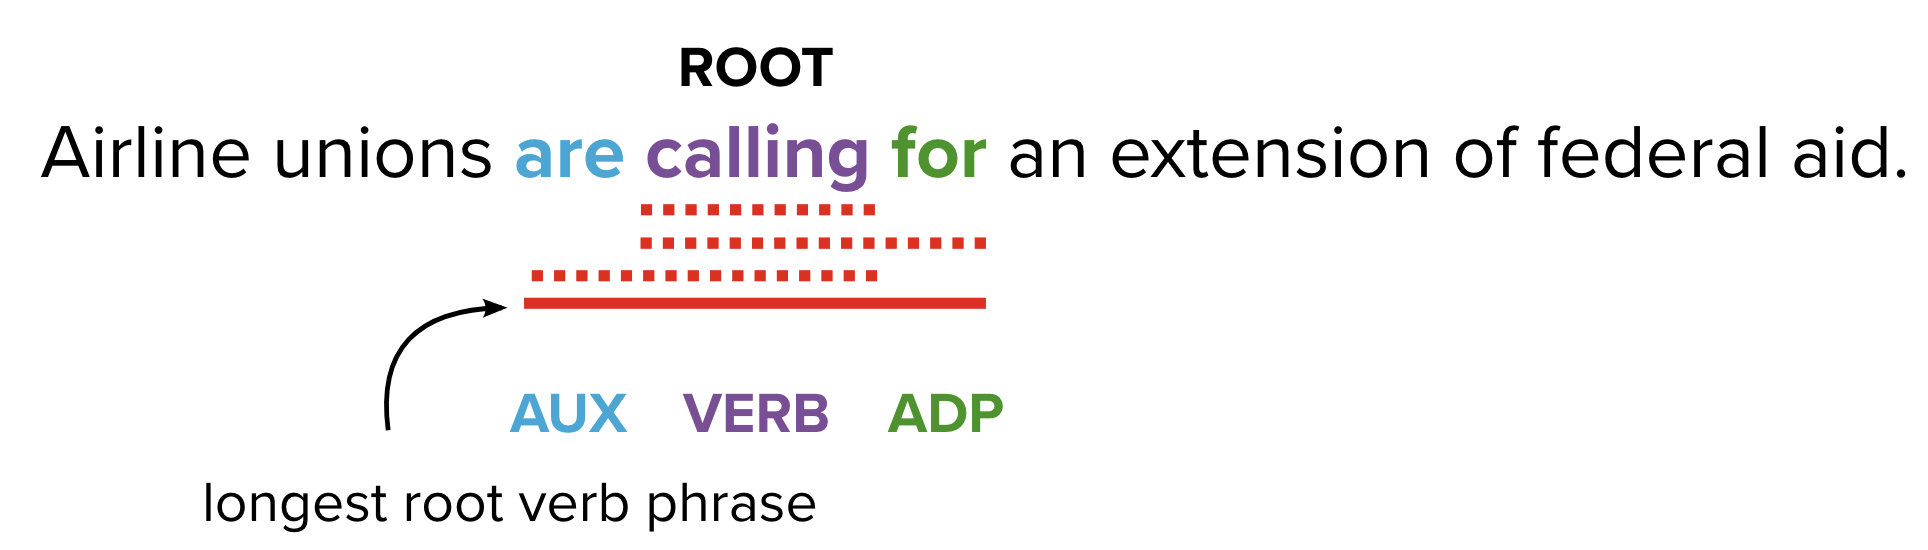
\includegraphics[scale=0.4]{images/verb_phrases.png}
\caption{Verb phrases extracted from an example sentence from article corpora}
\label{verb_phrases}
\end{figure}

% \begin{algorithm}
% \caption{My algorithm}
% \begin{algorithmic}[1]
% \Procedure{MyProcedure}{}
% \State $\textit{stringlen} \gets \text{length of }\textit{string}$
% \State $i \gets \textit{patlen}$
% \If {$i > \textit{stringlen}$} \Return false
% \EndIf
% \State $j \gets \textit{patlen}$
% \If {$\textit{string}(i) = \textit{path}(j)$}
% \State $j \gets j-1$.
% \State $i \gets i-1$.
% \State \textbf{goto} \emph{loop}.
% \State \textbf{close};
% \EndIf
% \State $i \gets i+\max(\textit{delta}_1(\textit{string}(i)),\textit{delta}_2(j))$.
% \State \textbf{goto} \emph{top}.
% \EndProcedure
% \end{algorithmic}
% \end{algorithm}

\subsection{Extracting Noun Phrases}

After the extracting the verb phrases for relations, the same is done for noun phrases in the sentences. As discussed in key decisions in order to capture meaningful relation, the model focuses on extracting subjects and objects as nouns. The most common sentence structure follows the dependency of subject-relation-object in that order. Therefore, for the scope of this project, the focus is directed to these types of semantic relations. First and foremost, for each sentence, the noun phrases are extracted in that sentence which uses chunking and POS-tagging exposed by SpaCy. These return a list of \texttt{Spans}, which are essentially slices of the sentence and contain information such as start, end position are of the phrase (slice) in teh sentence. Additionally, for each sentence all the relevant named entities are also extracted using the Fine-Grained NER model. These entities allowed all types such as 'GPE,' 'PER', 'LOC', 'ORG', 'NORP' etc. except for 'DATE', TIME', 'CARDINAL', 'PERCENT' and 'QUANTITY' \hl{(See Appendix for reference)}. This reason for this was the for each article corpus associated with a topic, the aim was to find information about named entities and how they related to one another. In particular, the model enforces the subject node to be about an entity. Therefore, including entity types such as 'DATE' for instance, can result in unnecessary and irrelevant triples with ('two', 'CARDINAL') as the subject node. This is not to say that any information about 'DATE', 'QUANTITY' etc. is completely ignored. Phrases containing these types of entities often show up object nodes when they are reference to a 'valid' subject named entity. 

\textbf{A base noun phrase, or “NP chunk”, is a noun phrase that does not permit other NPs to be nested within it, so no NP-level coordination, no prepositional phrases, and no relative clauses. copied from spacy doc}

\subsubsection{Subject phrases}

\todonum[inline]{Mad convoluted - rewrite}
In order to obtain the subject phrases, the noun phrases (returned as a list of Spans) are filtered to obtain those that have a starting position less than the starting position of the verb phrase as seen in line 5 in \ref{subject_phrase}. This essentially results in all noun phrases that are at the left of the root verb phrase. Additionally, as mentioned in Section \ref{subject_ents} since the subject node is enforced to be a valid entity, the noun phrases are filtered to obtain candidate subject phrases (\texttt{valid\_ents}) that mention a valid entity from the ones extracted from the sentence. From these candidate subject phrases, we obtain the first occurring (based on position of span) qualifying phrase as the subject phrase (lines 9-10). As seen in \ref{subject_phrase} on line 11, once the first qualifying phrase (i.e. entity) is found, the subject noun phrase is split to obtain the entity (which is the subject)  and the remnant phrase which gets prepended to the verb phrase to form the updated relation phrase. This way the information conveyed by the noun phrase is conserved but the subject nodes are maintained as an entity so a connected knowledge graph can be formed indicating the entity as the subject and showing relationships between these entities and relationships to other object nodes. 

\begin{listing}[H]
\caption{Get subject and relation}
\label{subject_phrase}
\begin{minted}[linenos]{python}
def get_subject_relation(verb_phrase, noun_phrases, ents):
  subject = None
  relation = None
  for n in noun_phrases:
    if n.start < verb_phrase.start:
      valid_ents = [(i,n.text.find(i)) for i in ents if n.text.find(i) != -1]
      if len(valid_ents) == 0:
        continue
      valid_ents.sort(key=lambda tup: tup[1])
      subject = valid_ents[0][0]
      relation = n.text.partition(subject)[2].strip() + ' ' + verb_phrase.text
      break
  return subject, relation
\end{minted}
\end{listing}

\subsubsection{Get object phrase}
The object phrase is also derived from the noun chunks in the sentence but instead of filtering the noun phrases occuring before the root verb phrase, the candidate object phrases obtained by finding all noun phrases (spans) where their starting position in the sentence is after the root verb phrase.

This particular method avoids the stringent dependency of the "subject" and "object" phrases on their actual dependency positions in the grammar, This is because given the nature of news articles, the sentence structure is relatively complex with several different subjects and objects. For the knowledge graph, ultimately, the relations extracted need to focus around different named entities. Relying on the dependency grammar structure to find the subject and object dos not hold as in a given sentence, the structure of the sentence heavily influences the information extracted. This means that more often than not, relevant information about entities is lost due to the entity not necessarily having one of \texttt{"nsubj", "csubj", "nsubjpass",	"csubjpass"} as the dependency. 

\todonum[inline]{Show types of relations extracted with dep parsing and otherwise}
\todonum[inline]{Talk about the object-relation-subject gotcha.}

\subsubsection{Filtering triples}
Once the semantic triples are obtained from the article corpus for each topic, the triples are filtered. After ensuring the that all components of the triple are not null, the triples where the relations/predicates contains words like "said" and "told" in their different forms are filtered. This is done because, often in news articles, direct quotes are made by entities and the relation extraction engine retrieves some poor relations that do not add to the quality of the relations extracted for a particular entity \hl{as seen in Figure} !!!! 

\todonum[inline]{Show some poor relations with said and told}

Once the qualifying semantic triples for each topic are obtained, these are passed to the visualisation engine. An example of the semantic relations extracted for the topics for a given cluster in Business 2021 is shown in \hl{Figure ??}